\graphicspath{{./friedman-test/img/}}
\chapter{Friedman's Test}
\label{C:friedman-test}
In this chapter we describe Friedman's approach to the two-sample
problem, give examples using a kernel support vector machine (KSVM), and
explain the connection between the KSVMs and the theory developed in
chapter~\ref{C:stein-proof}.

\section{Motivation}
The two-sample problem addresses the issue of comparing samples from
two possibly different probability distributions.  They range from
simple parametric, location alternative tests on univariate data such as the
$t$-test to more general non-parametric, asymptotically consistent tests, which
have power against all alternatives.  Many options exist for vectorial
data, and kernels provide an enticing avenue for extensions to more
general data types.

The two-sample problem is also widely prevalent: ensuring
cross-platform compability of microarray data allows for the merging
samples to achieve larger sample sizes.  Biologists would like to know
whether gene expression levels on a set of genes differ between cancer
and control groups.  Further uses for two-sample testing include
authorship validation: Given two sets of documents, is the hypothesis
of a single author consistent with the data?

\section{Two-Sample Tests}
The two-sample problem is generally posed in the following fashion: $\{
\mathbf{x}_i\}_1^n$ are drawn from $p(\mathbf{x})$ and
$\{\mathbf{y}_i\}_1^m$ are drawn from $q(\mathbf{y})$, where $\mathbf{x}_i,
\mathbf{y}_i \in \mathbb{R}^p$. The goal is to test $H_0:
p(\mathbf{x}) = q(\mathbf{y})$ against $H_A: p(\mathbf{x}) \neq
q(\mathbf{y})$. An ideal test should have power against all
alternatives. That is, as $n,m \to \infty$, the test
will always reject when $p \neq q$ for any non-zero significance level
$\alpha$.

There are many two-sample tests in the literature, as
Table~\ref{tab:twosampletests} illustrates.

\begin{table}
\centering
%\begin{tabular}{r|c|c|}
\begin{tabular}{r | p{5cm} | p{5cm} |}
\multicolumn{1}{r}{}
 & \multicolumn{1}{c}{parametric}
 & \multicolumn{1}{c}{non-parametric} \\
\cline{2-3}
univariate & $t$-test & permutation $t$-test; Kolmogorov-Smirnov
test; Wilcoxon rank-sum test \\
\cline{2-3}
multivariate & Hotelling's $T^2$ test & Friedman-Rafsky test \\
\cline{2-3}
non-vectorial & Maximum Mean Discrepancy (asymptotic) & Friedman's test (KSVM);
MMD (distribution-free) \\
\cline{2-3}
heterogeneous & & Friedman's test (MKL) \\
\cline{2-3}
\end{tabular}
\caption{Two-sample tests.}
\label{tab:twosampletests}
\end{table}

\section{The Friedman Two-Sample Test}
Friedman proposed the following approach to the two-sample problem
\cite{friedman30908multivariate}:

For $\{\mathbf{x}_i\}_1^N$ drawn from $p(\mathbf{x})$ and
$\{\mathbf{z}_i\}_1^M$ drawn from $q(\mathbf{x})$, we would like to
test $\mathcal{H}_A$: $p \neq q$ against $\mathcal{H}_0$: $p = q$.
\begin{enumerate}
\item Pool the two samples $\{\mathbf{u}_i\}_1^{N+M} =
  \{\mathbf{x}_i\}_1^{N} \cup \{\mathbf{z}_i\}_1^{M}$ to create a
  predictor variable training set.
\item Assign a response value $y_i = 1$ to the observations from the
  first sample ($1 \leq i \leq N$) and $y_i = -1$ to the observations
  from the second sample ($N + 1 \leq i \leq N+M)$.
\item Apply a binary classification learning machine to the training
  data to produce a scoring function $f(\mathbf{u})$ to score each of
  the observations $\{s_i = f(\mathbf{u}_i)\}_1^{N+M}$. \label{item:friedman-score}
\item Calculate a univariate two-sample test statistic $\hat{t} =
  T(\{s_i\}_1^N,\{s_i\}_{N+1}^{N+M})$.
\item Determine the permutation null distribution of the above
  statistic to yield a p-value.
\item The test rejects $\mathcal{H}_0$ at significance level $\alpha$
  if $p < \alpha$.
\end{enumerate}

Note that in step~\ref{item:friedman-score}, for a given learning
machine, there can still be some choice in the scoring function
$f(\mathbf{u})$.

The Friedman Test (FT) is a simple, elegant idea that leverages the
many advancements made over the past several decades in the fields of
prediction and classification and applies them to the problem of
two-sample testing.  In short, as long as there exists a learning
machine for the problem at hand, the Friedman Test provides a recipe
for turning that learning machine into a two-sample test.  This
immediately yields two-sample tests for many kinds of data, including
all types for which kernels have been defined.
But there still remains some choice in the scoring
function $F(\mathbf{u})$.  It must be flexible enough to discriminate
between the potential distributional differences of the problem at
hand.  The operating characteristics of the new two-sample test is
\emph{solely} a function of the paired learning algorithm.

By virtue of its permutation construction, the test has level $\alpha$---the
probability that we reject the null hypothesis given
that the null hypothesis is true, also known as type I error.  Given a
threshold $\alpha$, we wish to minimize the type II error, accepting
the null hypothesis given that the alternative hypothesis is true.
Equivalently, we wish to maximize the power, one minus the type II
error \cite{lehmann2005testing}.  The downside of the permutation
design is, of course, that any computational cost is na\"\i vely
multiplied by the number of permutations.  However, there are many
situations for which the cost is sublinear in the number of
permutations.  For instance, caching the computation of the kernel matrix
yields substantial savings when re-using it for permutation based
inference.  This is especially true when computation of the kernel
matrix is expensive relative to finding the SVM parameters via
quadratic programming.

The exact randomization distribution will be a complicated, discrete distribution
parametrized by the observed data.  If, however, we can approximate this
distribution with a simpler one and derive error bounds on the difference
between the two distributions in some probability metric, then we can
use the target distribution as a basis for inference.  We will gain in
computational efficiency by only having to compute the test statistic once.

\section{Kernel Methods}
There exist many two-sample tests for vectorial data $\mathbf{x}_i \in \mathbb{R}^p$.
Increasingly, data collected for many applications is heterogeneous in nature
and include non-vectorial components such as text, audio, or graph structures
for which the mathematical and geometric operations required of many learning
algorithms are not defined.  Kernel methods allow us to identify a mapping
of the data from a general set into a Hilbert space in which we can apply
certain classes of algorithms.  There is much literature on kernel methods,
but one particularly comprehensive treatment is the monograph by Sch{\"o}lkopf
and Smola \cite{scholkopf2002learning}.

Given $n$ observed datapoints in some general set, $x_1, \ldots, x_n \in \mathcal{X}$,
kernelized learning algorithms depend only on the pairwise ``similarities'' between
any two observations by way of the kernel function.  Thus, kernel methods effectively
decouple the algorithm (e.g. a support vector machine) from the representation
of the data (e.g. a particular kernel).
\begin{definition}[Positive Semidefinite Kernel]
\label{D:kernel}
A function $K: \mathcal{X} \times \mathcal{X} \to \mathbb{R}$ is called a positive
semidefinite kernel iff it is symmetric ($K(x, x') = K(x', x)$ for any
$x, x' \in \mathcal{X}$) and positive semidefinite:
\begin{equation*}
  \sum_{i=1}^n\sum_{j=1}^nc_ic_jK(x_i, x_j) \geq 0
\end{equation*}
for any $n > 0$, any choice of $n$ objects $x_1, \ldots, x_n \in \mathcal{X}$,
and any $c_1, \ldots, c_n \in \mathbb{R}$.
\end{definition}

Because inner products are symmetric, positive semidefinite functions, they
satisfy Definition~\ref{D:kernel} and are valid kernels.  When $\mathcal{X} = \mathbb{R}^p$,
the linear kernel is defined as
\begin{equation*}
  K(\mathbf{x}, \mathbf{x'}) = \langle \mathbf{x}, \mathbf{x'} \rangle
\end{equation*}
for $\mathbf{x}, \mathbf{x'} \in \mathcal{X}$.

For objects in general sets $\mathcal{X}$, we can define a mapping $\phi$ into a
Hilbert space $\mathcal{H}$ for which an inner product exists.  As there are
many such mappings, one challenge is to choose a one that is maximally
useful in exploiting the structure of the data for the task at hand.  In
Chapter~\ref{C:MKL}, we shall explore a technique to identify the most useful
mapping given some parametrized space of mappings.

In fact, for every kernel $K$ we can identify a feature mapping into a Hilbert
space, where the kernel can be expressed as the inner product of the mapped
features \cite{scholkopf2004kernel}:
\begin{theorem}
  For any kernel $K: \mathcal{X} \times \mathcal{X} \to \mathbb{R}$, there
  exists a Hilbert space $\mathcal{H}$ and a feature mapping
  $\phi: \mathcal{X} \to \mathcal{H}$ such that
  \begin{equation*}
    K(x, x') = \langle \phi(x), \phi(x') \rangle_{\mathcal{H}}
  \end{equation*}
  for any $x, x' \in \mathcal{X}$, where $\langle u, v \rangle_{\mathcal{H}}$
  represents the inner product in $\mathcal{H}$.
\end{theorem}

In the coming sections and in Chapter~\ref{C:MKL}, we shall see examples of
nonvectorial spaces $\mathcal{X}$, kernels $K$, feature mappings $\phi$, and
Hilbert spaces $\mathcal{H}$.

\section{Support Vector Machines}
Support Vector Machines (SVM) \cite{cortes1995support} are a supervised learning
technique that seeks to find a hyperplane that maximizes the margin between
points of different classes.  In the case that there exists no separating
hyperplane, a regularization term can be added that controls the effect of
misclassified points.

Although SVMs find linear decision boundaries,
the algorithm depends only on inner products between its datapoints.  The
``kernel trick'' \cite{aizerman1964theoretical} allows us to replace the
inner products with kernel function evaluations, thus effectively identifying
a linear decision boundary in the Hilbert space $\mathcal{H}$ identified by
the feature mapping $\phi(x): \mathcal{X} \to \mathcal{H}$.  Although linear
in the typically-higher-dimensional space $\mathcal{H}$, the decision boundary
can be nonlinear in $\mathcal{X}$.

Since kernel methods divorce the representation of the data with the learning
algorithm, development on both fronts can proceed independently.  For instance,
faster optimization algorithms for solving the general SVM problem can proceed
in parallel with the problem-specific designing of new kernels to more efficiently
or effectively exploit the structure of the data.

Consider the $\ell_1$-regularized (soft margin) support vector classification
problem \cite{scholkopf2002learning} in its primal form:
\begin{equation}
\label{eq:l1-svm-primal}
\begin{aligned}
& \underset{\mathbf{w} \in \mathcal{H}, b \in \mathbb{R}, {\boldsymbol \xi} \in \mathbb{R}^m}{\text{minimize}}
& &\frac{1}{2}\norm{\mathbf{w}}_2^2+C\sum_{i=1}^m \xi_i \\
& \text{subject to}
& & y_i(\mathbf{w}^t \mathbf{x}_i + b) \geq 1 - \xi_i \\
&&& \xi_i \geq 0 \qquad \qquad \quad \text{for all } i=1,\ldots,m.
\end{aligned}
\end{equation}

There are three obvious possibilities for the Friedman scoring
function $f$:
\begin{enumerate}
\item The predicted class label $f_1(\mathbf{x}_i)
= \text{sign}(\mathbf{w}^t \mathbf{x}_i + b)$.
\item An estimate of the posterior class probability, such as by a
sigmoid (Platt \cite{platt1999probabilistic, lin2007note}) or a
logistic link function (Wahba \cite{wahba1992multivariate,
wahba1999support})
$f_2(\mathbf{x}_i) = \frac{1}{1 + \text{exp}(-(\mathbf{w}^t \mathbf{x}_i + b))}$.
\item The margin $f_3(\mathbf{x}_i) = \mathbf{w}^t \mathbf{x}_i + b$.
\end{enumerate}

Because the predicted class label is simply the sign of the margin, we
lose information about how likely it is for a given observation
to belong to a particular class.  Moreover, given constant within-class
predicted class labels, the sample standard deviation is $0$ and hence
the $t$-statistic is unbounded.

Using, for instance, a logistic link function, $f_2$ has the
interpretability of being a posterior class probability (if you
believe in the probability model) and yields no information loss
(since it is simply an invertible function of the margin).  However,
it is typically not a linear function of the margin.

The margin $f_3$ has the advantage of being an affine function of the
data.  In one dimension, $f_3(x_i) = w x_i + b$, and since the
$t$-statistic is invariant (up to sign) to affine transformations of
the data, we can see that using the margin generalizes the permutation
$t$-test in some sense.

In the univariate setting, whether or not the $t$-statistic computed
on the scores $\{f_3(x_i)\}$ agrees with that on the raw data
$\{x_i\}$ depends on $\text{sign}(w)$.  Due to symmetry, in the
permutation null distribution, $w$ is negative with probability $.5$
and positive with probability $.5$.  Thus, the permutation null in
both settings appears to be $t$ (and hence asymptotically normal).

\subsection{Kernelized Form}
It is advantageous to treat the dual \cite{boyd2004convex} of
Problem~(\ref{eq:l1-svm-primal}).  Because of strong duality,
the primal and dual solutions are equivalent.
Although both optimization problems
are quadratic programs, there exist fast algorithms such as the
sequential minimal optimization algorithm \cite{platt199912} that
exploit the special structure of the dual problem.

In addition, the dual problem is expressed only in terms of inner
products, $\langle \mathbf{x_i}, \mathbf{x_j} \rangle$.  The kernel trick
\cite{aizerman1964theoretical} amounts to replacing these inner products
with kernel function evaluations, $K(\mathbf{x_i}, \mathbf{x_j})$.  The
dual optimization problem is given by
\begin{equation}
\label{eq:l1-svm-dual}
\begin{aligned}
& \underset{{\boldsymbol \alpha} \in \mathbb{R}^m}{\text{minimize}}
& & \sum_{i=1}^m \alpha_i - \frac{1}{2} \sum_{i,j=1}^m \alpha_i \alpha_j y_i y_j K(\mathbf{x_i}, \mathbf{x_j})  \\
& \text{subject to}
& & 0 \leq \alpha_i \leq C \quad \text{for all } i=1,\ldots,m \\
& \text{and}
& & \sum_{i=1}^m \alpha_i y_i = 0.
\end{aligned}
\end{equation}

The Karush--Kuhn--Tucker (KKT) conditions for optimality imply that
\begin{equation*}
  \mathbf{w} = \sum_{i=1}^m \alpha_i y_i \mathbf{x}_i.
\end{equation*}
Therefore,
\begin{equation*}
  f(\mathbf{x}) = \mathbf{w}^T\mathbf{x} + b = \sum_{i=1}^m \alpha_i k(\mathbf{x}, \mathbf{x}_i) + b.
\end{equation*}

In fact, there is another view of the SVM problem in the framework of regularized
empirical risk minimization that will be useful for Chapter~\ref{C:MKL}.
Define the hinge loss function
\begin{equation*}
  L(y, f(x)) := (1 - yf(x))_+ := \max(0, 1 - yf(x)).
\end{equation*}
Then the following optimization problem is equivalent to Problem~(\ref{eq:l1-svm-primal}):
\begin{equation}
  \label{eq:hinge-svm}
  \min_{b \in \mathbb{R}, \mathbf{w} \in \mathcal{H}} \sum_{i=1}^m (1 - y_i(\mathbf{w}^T\mathbf{x}_i + b))_+ +
  \frac{1}{2C} \norm{\mathbf{w}}_2^2.
\end{equation}

It turns out that regularized risk minimization problems admit particularly elegant
solutions, a result owing to Kimeldorf and Wahba \cite{kimeldorf1971some}.  We
present a slightly generalized representer theorem from \cite{scholkopf2002learning}:
\begin{theorem}[Representer Theorem]
  \label{T:representer}
  Let $\Omega:[0, \infty] \to \mathbb{R}$ be a strictly monotonic increasing function,
  $\mathcal{X}$ be a set, and $c: (\mathcal{X} \times \mathbb{R}^2)^m \to \mathbb{R} \cup \{\infty\}$
  be an arbitrary loss function.  Then each minimizer $f \in \mathcal{H}$ of the regularized risk
  \begin{equation*}
    c((\mathbf{x_1}, y_1, f(\mathbf{x_1})), \ldots, (\mathbf{x_m}, y_m, f(\mathbf{x_m}))) + \Omega(\norm{f}_{\mathcal{H}})
  \end{equation*}
  admits a representation of the form
  \begin{equation*}
    f'(\mathbf{x}) = \sum_{i=1}^m \alpha'_i k(\mathbf{x}_i, \mathbf{x}).
  \end{equation*}
\end{theorem}

We apply Theorem~\ref{T:representer} to Problem~(\ref{eq:hinge-svm}), noting that it holds
for all fixed $b$, to conclude that
\begin{equation*}
  f'(\mathbf{x}) = \mathbf{w}^T\mathbf{x} = \sum_{i=1}^m \alpha'_i k(\mathbf{x}_i, \mathbf{x}).
\end{equation*}
Thus, setting $\alpha'_i = y_i \alpha_i$, we again find
\begin{equation*}
  f(\mathbf{x}) = f'(\mathbf{x}) + b = \sum_{i=1}^m y_i \alpha_i k(\mathbf{x}, \mathbf{x}_i) + b.
\end{equation*}

We list the kernelized representations of possible Friedman scoring functions:
\begin{enumerate}
\item The predicted class label $f_1(\mathbf{x}_i)
= \text{sign}(\sum_{i=1}^m y_i \alpha_i k(\mathbf{x}, \mathbf{x}_i) + b)$.
\item An estimate of the posterior class probability, such as by a
sigmoid (Platt \cite{platt1999probabilistic, lin2007note}) or a
logistic link function (Wahba \cite{wahba1992multivariate,
wahba1999support})
$f_2(\mathbf{x}_i) = \frac{1}{1 + \text{exp}(-(\sum_{i=1}^m y_i \alpha_i k(\mathbf{x}, \mathbf{x}_i) + b)}$.
\item The margin $f_3(\mathbf{x}_i) = \sum_{i=1}^m y_i \alpha_i k(\mathbf{x}, \mathbf{x}_i) + b$.
\end{enumerate}

We know that in the univariate setting, we have an equivalence to the
permutation $t$-test as long as the margin is an affine function of
the data.  So, for what kernels $k$ do we have
\begin{equation}
\sum_{i=1}^m y_i \alpha_i k(x, x_i) + b = cx + d?
\end{equation}

A sufficient condition is for $k(x, x_i) = \langle \Phi(x), \Phi(x_i) \rangle =
f(x_i) x$.  The linear kernel satisfies this condition with $f(x_i) =
x_i$.  The RBF kernel $k(x, x_i) = \text{exp}(-\sigma (x-x_i)^2)$ does
not yield an affine function of the data:
\begin{equation}
\sum_{i=1}^m y_i \alpha_i \text{exp}(-\sigma (x-x_i)^2) + b
\end{equation}
cannot be written as $cx + d$.

We use Support Vector Machine (SVM) classification
as implemented in the {\bf ksvm} function of the {\bf R}
\cite{cran} package {\bf kernlab} \cite{kernlab}.

SVM regression scores also generalize the permutation $t$-test.
Recall that SVM regression solves the following problem \cite{scholkopf2002learning}:
\begin{equation*}
\begin{aligned}
& \underset{\mathbf{w}\in\mathcal{H},\mathbf{\xi}^{(*)}\in\mathbb{R}^m,b\in\mathbb{R}}{\text{minimize}}
& &\tau(\mathbf{w},\mathbf{\xi}^{(*)})=\frac{1}{2}\norm{\mathbf{w}}^2+C\sum_{i=1}^M(\xi_i+\xi_i^*) \\
& \text{subject to}
& & f(\mathbf{x}_i)-y_i \leq \epsilon +\xi_i\\
&&& y_i-f(\mathbf{x}_i) \leq \epsilon+\xi_i^* \\
&&& \xi_i,\xi_i^*\geq0 \qquad \qquad \quad \text{for all } i=1,\ldots,m.
\end{aligned}
\end{equation*}
with solution is given by
\begin{equation*}
  f(x)=\sum_{i=1}^m(\alpha_i^*-\alpha_i)k(x_i,x)+b.
\end{equation*}
\subsection{Tuning Parameters}

The cost parameter $C$ controls the complexity of the prediction
function, and $\epsilon$ controls the leniency of the loss function.
These parameters are typically chosen via cross-validation over a grid
of choices.  In subsection~\ref{twitter_data}, we describe a sample of
string data from Twitter.  In figure~\ref{fig:power_kpar} we
demonstrate the statistical power of the test for the Twitter data
over a grid of SVM parameters.  It is clear that these parameters play
a \emph{crucial} role in the operating characteristics of the
resultant test.

We emphasize that the proper strategy is to conduct the search anew
for each statistic calculation in each permutation.  That is, use cross-validation to
find the best performing pair $(C_0, \epsilon_0)$ in terms of the
Friedman Statistic.  For each permutation $i$, use cross-validation
over the same grid to find the $i$th pair $(C_i, \epsilon_i)$.  This
ensures symmetry of protocol and enforces that the test have level
$\alpha$.  The grid search likely maximizes the power over the set of
tuning parameters: it is hoped that the search benefits the actual
labeling of values by at least as much as it does permuted labels.

\subsection{Equivalence to the Permutation $t$-test}
\begin{theorem}
  \label{friedman_equiv}
  The Friedman Test paired with support vector regression
  or support vector classification (using the margin as a score)
  with the appropriate kernel generalizes
  the two-sample permutation $t$-test. Namely, the two procedures are
  equivalent with univariate data and a linear kernel.
\end{theorem}

\begin{proof}
  \begin{equation*}
    f(x)=\sum_{i=1}^m(\alpha_i^*-\alpha_i)k(x_i,x)+b =
    \sum_{i=1}^m(\alpha_i^*-\alpha_i)x_ix+b = wx+b
  \end{equation*}
  since we have univariate data and a linear kernel.
  Therefore, the SVM score is simply a linear transformation of the
  data.  Welch's $t$-statistic is given by
  \begin{equation*}
    T(\{x_i\}_1^N,\{z_i\}_1^M) = \frac{\bar{x}-\bar{z}}{\sqrt{\frac{s_X^2}{N}+\frac{s_z^2}{M}}}
  \end{equation*}
  where
  \begin{equation*}
    \bar{x}=\frac{1}{N}\sum_{i=1}^N x_i \text{ and }
    s_X^2= \frac{1}{N-1}\sum_{i=1}^N(x_i-\bar{x})^2.
  \end{equation*}
  Let $z=f(x)=wx+b$ and note that
  \begin{equation*}
    \bar{z}=\frac{1}{N}\sum_{i=1}^N z_i = \frac{w}{N}\sum_{i=1}^N x_i
    + b = w\bar{x}+b
  \end{equation*}
  and
  \begin{equation*}
    s_Z^2= \frac{1}{N-1}\sum_{i=1}^N(z_i-\bar{z})^2= \frac{1}{N-1}\sum_{i=1}^N(wx_i+b-w\bar{x}+b)^2=w^2s_X^2.
  \end{equation*}
  Therefore,
  \begin{equation*}
    T(\{f(x_i)\}_1^N,\{f(z_i)\}_1^M) =
    \frac{w\bar{x}+b-w\bar{z}+b}{|w|\sqrt{\frac{s_X^2}{N}+\frac{s_z^2}{M}}}
    = \text{sign}(w) T(\{x_i\}_1^N,\{z_i\}_1^M).
  \end{equation*}
  Since we are interested in two-sided testing, we consider
  \begin{equation*}
    |T(\{f(x_i)\}_1^N,\{f(z_i)\}_1^M)| = |T(\{x_i\}_1^N,\{z_i\}_1^M)|.
  \end{equation*}
  Thus, the $t$-statistics are identical, and since the permutation
  procedure is the same, the tests are equivalent.
\end{proof}

Despite the slight dependence, the randomization distribution of the
$t$-statistic converges weakly to the normal distribution
\cite{lehmann1999elements}.  Anonymous and Anonymous \cite{rayholmes2012} use
Stein's Method of exchangeable pairs \cite{chen2010normal,
  stein1986approximate} to prove a conservative
$\mathcal{O}(N^{-1/4})$ rate of convergence in Kolmogorov-Smirnov
distance between the two distributions.  The problem is not as
straightforward as in the i.i.d. case because the permutation
structure induces a global---though mild and diminishing in sample
size---negative dependence in the data.  This dependence thwarts
traditional Fourier-analytic techniques yet can be managed via Stein's
eponymous method of proof.

\section{Maximum Mean Discrepancy}
Gretton et al.\ \cite{gretton19m, gretton2010fast, gretton2012kernel,
  borgwardt2006integrating} introduce a kernel based approach for
the two-sample problem based on the Maximum Mean Discrepancy (MMD)
statistic, an integral probability metric.  MMD provides good
performance in practice, strong theoretical guarantees, and is the
first two-sample test for comparing distributions over graphs.

\begin{definition}
  With $\mathfrak{F}$ a class of functions $f:\mathcal{X} \to
  \mathbb{R}$, $p$ and $q$ probability distributions, and $X \sim p$
  and $Z \sim q$ random variables, the maximum mean discrepancy (MMD)
  and its empirical estimate are defined as
  \begin{equation*}
    \text{MMD}[\mathfrak{F},p,q] := \sup_{f\in
      \mathfrak{F}}(\mathbb{E}_{x\sim p}[f(x)] - \mathbb{E}_{z\sim q}[f(z)]),
  \end{equation*}
  \begin{equation*}
    \text{MMD}[\mathfrak{F},X,Z] := \sup_{f\in
      \mathfrak{F}}\left (\frac{1}{N}\sum_{i=1}^Nf(x_i) -
    \frac{1}{M}\sum_{i=1}^M f(z_i) \right ).
  \end{equation*}
\end{definition}

The function class $\mathfrak{F}$ is typically taken to be the unit ball in a
reproducing kernel Hilbert space (RKHS), however, well-known metrics
can be obtained over other function classes.  Although Gretton et
al.\ provide several distribution-free tests based on MMD theory, we
instead compare the Friedman Test (FT) against the permutation-based
MMD so as to compare statistic with statistic.  In this way, the
theory is dissociated from the comparison.  We feel that this is the
most fair comparison of the two tests because many of the theoretical
results are inexact.  We also do not have big enough sample sizes in
our real datasets to ensure low error in theoretical approximations.
Even if we did, the power for the tests would be very nearly one,
making comparisons on non-simulated data difficult.

\section{Null Distributions}
The null distribution plays a fundamental role in frequentist statistical
inference.  Hotelling's $T^2$-statistic has null distribution that
corresponds to a scaled central $F_{(p, n+m-1-p)}$ distribution, where
$p$ is the dimensionality of the data and $n, m$ are the sample sizes
of the two groups.  As its name suggests, the $T^2$-test is a
generalization of Student's $t$-test, and for $T \sim t(n+m-2)$, we
have that $T^2 \sim F_{(1, n+m-2)}$.  As a consequence of
Theorem~\ref{friedman_equiv}, the Friedman Statistic in the univariate
data, linear kernel setting is equal to the $|T|$.  In figure~\ref{fig:null_dist} we simulate
200 standard multivariate normal draws from each class with dimension
$D \in \{1, 5, 10\}$.  We compare the null distributions of the
$T^2$-statistic, KMMD, and Friedman statistics with a linear kernel
and RBF kernel with width parameter 1.  We draw 5,000 samples from
each permutation null distribution and apply a kernel density smoother
to the results.  It appears that many of the null distributions are
very close to Normal (or, $t(398)$, rather).

Observe the Anderson-Darling test for normality $p$-values for each
statistic:
\begin{verbatim}
    D variable            p-value
1   1       T2           NaN
2   1   sqrtT2 1.152257e-157
3   1   KMMD.l 2.659966e-156
4   1     FS.l  9.210211e-01
5   1 KMMD.rbf  2.220671e-84
6   1   FS.rbf  7.945208e-01
7   5       T2 1.750434e-156
8   5   sqrtT2  1.320034e-14
9   5   KMMD.l  4.955331e-39
10  5     FS.l  2.908307e-03
11  5 KMMD.rbf  1.475365e-15
12  5   FS.rbf  5.837144e-01
13 10       T2 5.660731e-105
14 10   sqrtT2  4.132584e-11
15 10   KMMD.l  4.087932e-38
16 10     FS.l  7.618190e-01
17 10 KMMD.rbf  3.778002e-01
18 10   FS.rbf  8.071885e-01
\end{verbatim}

Now only $p$-values $> .001$:
\begin{verbatim}
    D variable            p-value
4   1     FS.l 0.921021148
6   1   FS.rbf 0.794520826
10  5     FS.l 0.002908307
12  5   FS.rbf 0.583714415
16 10     FS.l 0.761819040
17 10 KMMD.rbf 0.377800181
18 10   FS.rbf 0.807188534
\end{verbatim}

The Friedman Statistic null distributions appear to be consistent with
a standard Normal distribution.

Note that in one dimension, the $t$-statistic is independent of the
regularization parameter $C$.  This relationship does not hold in
higher dimensions:
\begin{verbatim}
laply(10^seq(-3, 3, 1), function(C) computeFS(u, km, l, C)) ## 1 dimension
> [1] 0.6438212 0.6438212 0.6438212 0.6438212 0.6438212 0.6438212 0.6438212
laply(10^seq(-3, 3, 1), function(C) computeFS(u, km, l, C)) ## 2 dimensions
> [1] 3.172028 3.172028 3.174125 3.168278 3.172856 3.169756 3.169530
laply(10^seq(-3, 3, 1), function(C) computeFS(u, km, l, C)) ## 10 dimensions
> [1] 6.830184 6.850385 6.034328 6.619036 6.619036 6.619036 6.619036
\end{verbatim}
This suggests that $C$ actually has an influence in higher dimensions.

\begin{figure}
\centering
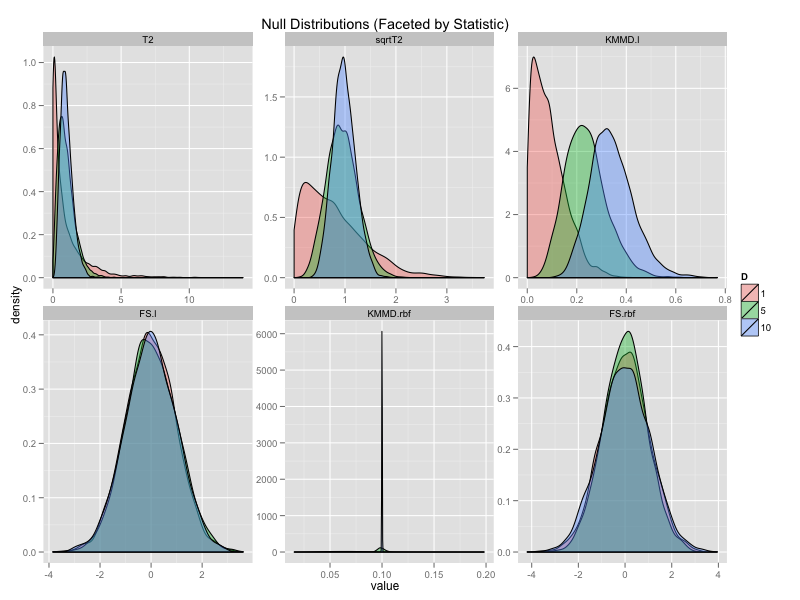
\includegraphics[width=.8\linewidth]{null_dist.png}
\caption{T2: Hotelling's $T^2$-statistic; sqrtT2: $|T|$;
KMMD.l: kernel MMD with a linear kernel; FS.l: FS with a
linear kernel; KMMD.rbf: kernel MMD with a radial basis function (RBF) kernel;
FS.rbf: FS with RBF kernel}
\label{fig:null_dist}
\end{figure}

The $T^2$ densities correspond to a
parametrized family of $F$-distributions.  It is not surprising that the MMD
linear kernel null distributions shift rightward as a function of
dimension: the higher dimensionality affords the function in the RKHS
to better find discrepancies between the two empirical distributions.
The same rationale holds true for the FS when thinking of separating
hyperplanes.  Interestingly, there are marked differences between the
MMD and FS for the RBF kernel.

\section{Experiments}
\subsection{Vectorial Data}
We consider $\{x_i\}_{i=1}^{20} \sim \mathrm{MVN}_d(\mathbf{0},
\mathbf{I})$ and $\{y_i\}_{i=1}^{20} \sim
\mathrm{MVN}_d(\Delta \mathbf{1}, \mathbf{I})$ where our
dimensionality $d \in \{1, 5, 10, 20\}$ and mean difference $\Delta \in
\{0, .5, \ldots, 1.5\}$ in figure~\ref{fig:power_normal}.  The width
parameter in the RBF kernel is fixed at 1.

\begin{figure}
  \centering
  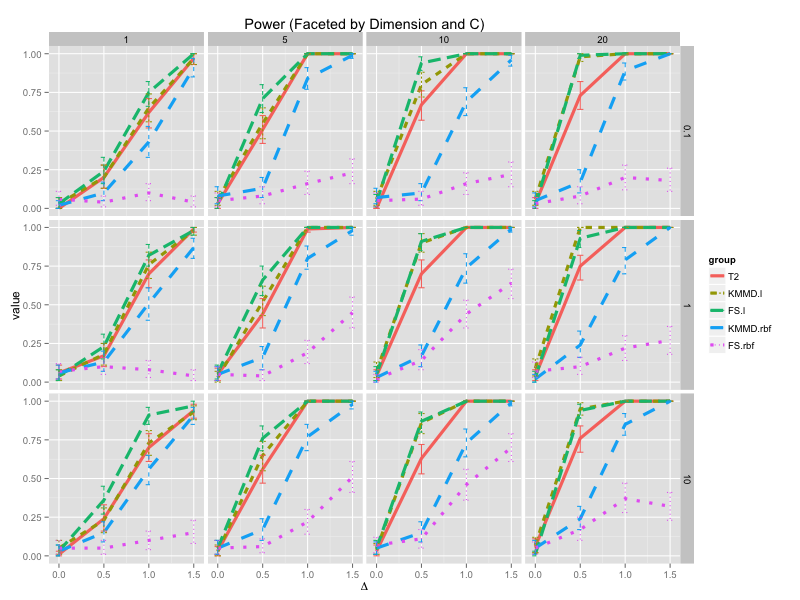
\includegraphics[width=\linewidth]{power_normal.png}
  \caption{FS: Friedman statistic; KMMD: kernel Maximum Mean
    Discrepancy; T2: Hotelling's $T^2$-statistic; Error bars indicate
    95\% bootstrap confidence intervals.  The tests perform similarly,
    and the kernel-based tests use a linear kernel.}
  \label{fig:power_normal}
\end{figure}

For FS and MMD, we used the the RBF kernel with a width of 1.  The
methods perform similarly with the exception of the kernel methods
using the RBF kernel.  This suggests that either a width of 1 is
ineffective or the RBF kernel is unsuitable for these data (probably the former).

\subsection{String Data}
\label{twitter_data}
For a string data comparison, we consider Twitter data and look at the
latest 1,000 tweets from Barack Obama (@BarackObama) and Sarah Palin
(@SarahPalinUSA) obtained from the \bf{R} package \bf{twitteR}
\cite{twitteR}.  We pre-process each tweet by removing all
hyperlinks and anything that is neither a letter nor a space.
Finally, we convert all letters to lowercase.  For simplicity, we
choose the $k$-spectrum kernel \cite{leslie2002spectrum} with
$k \in \{1, 2, 3 \}$
as our kernels for both the FT and MMD.  Thus, each string is mapped to
a $27^k$ dimensional feature vector of counts of the number of $k$
letter and space combinations.  We draw samples of various sizes from
both the Barack Obama tweets and Sarah Palin tweets in order to
empirically determine the power, with results detailed in
figure~\ref{fig:power_string}.

\begin{figure}
  \centering
  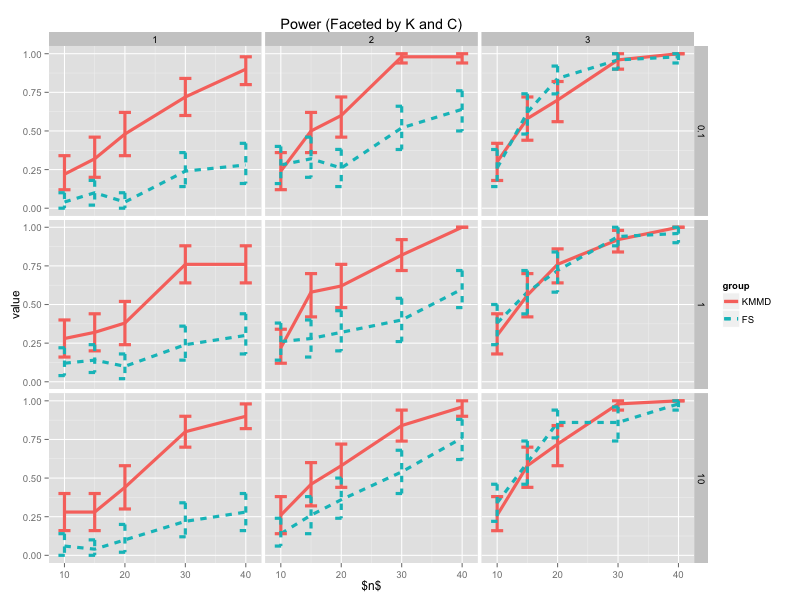
\includegraphics[width=\linewidth]{power_string.png}
  \caption{FS: Friedman statistic; KMMD: kernel Maximum Mean
    Discrepancy; Error bars indicate 95\% bootstrap confidence
    intervals.}
  \label{fig:power_string}
\end{figure}

The MMD test outperforms the Friedman test on this task for $k < 3$.  Power
increases as a function of $k$ for both tests, and it is somewhat
surprising to see the strong performance from considering only
frequencies of unigrams.

\subsection{Image Data}
\begin{figure}
  \centering
      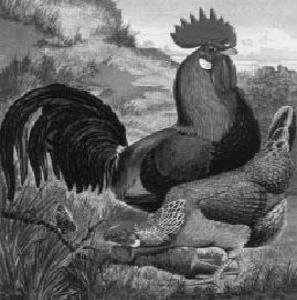
\includegraphics[scale=.2]{roosterrs-image_0001.jpg}
      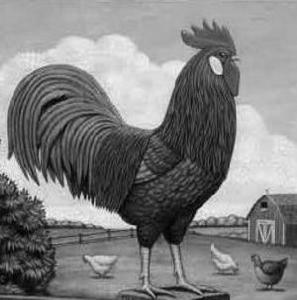
\includegraphics[scale=.2]{roosterrs-image_0002.jpg}
      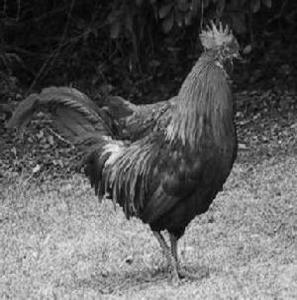
\includegraphics[scale=.2]{roosterrs-image_0003.jpg}
      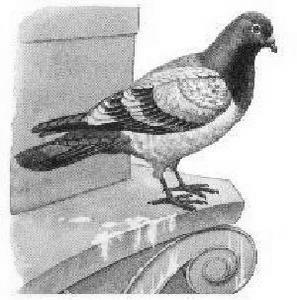
\includegraphics[scale=.2]{pigeonrs-image_0001.jpg}
      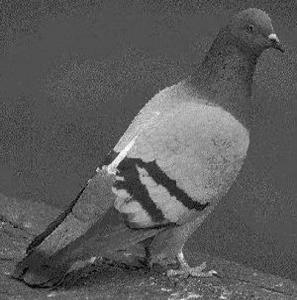
\includegraphics[scale=.2]{pigeonrs-image_0002.jpg}
      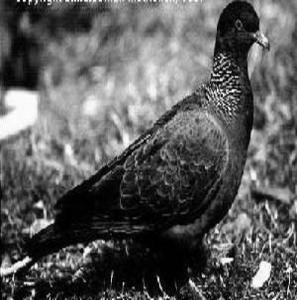
\includegraphics[scale=.2]{pigeonrs-image_0004.jpg}
      \caption{Images of roosters and pigeons for use in
        discrimination test.}
  \label{fig:birds}
\end{figure}

We consider the task of discriminating between images of roosters and
pigeons from the Caltech 101 Object Categories dataset
\cite{fei2007learning}.  Samples of the birds are in figure~\ref{fig:birds}.
We resize images to a common resolution of $300 \times
297$ and convert to a vector of 8 bit grayscale values.
To correct for global differences in illumination and ensure
that only local patterns would be used for discrimination, we center and
scale each vector.  Power comparisons can be seen in figure~\ref{fig:power_birds}.

\begin{figure}
  \centering
  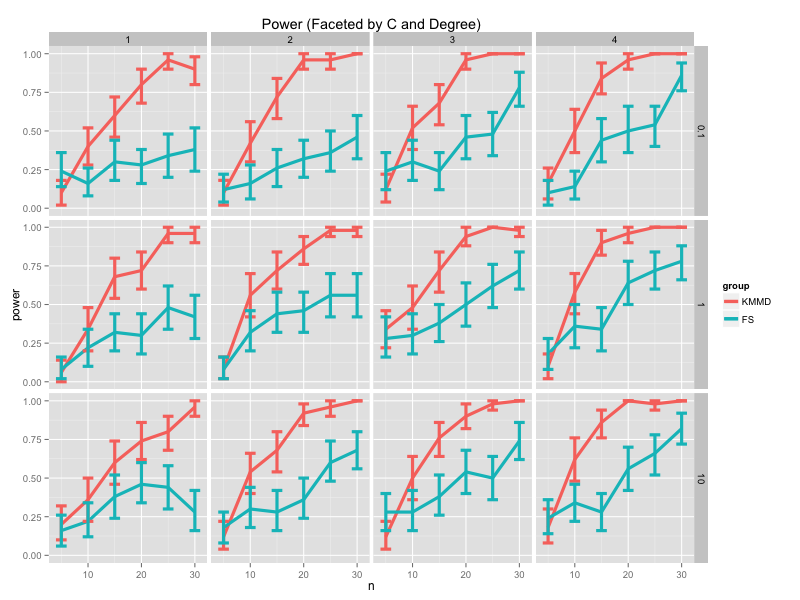
\includegraphics[width=\linewidth]{power_birds.png}
  \caption{p1: linear kernel; p2: inhomogeneous degree 2 polynomial
    kernel; rbf: radial basis function kernel; Error bars indicate
    95\% bootstrap confidence intervals.}
  \label{fig:power_birds}
\end{figure}

Again, MMD performs better.  However, it appears that the linear
kernel performs significantly worse for the MMD than for the FS.
This could reflect a difference in the function classes over which
each technique operates.

\section{Extensions}
\subsection{Heterogeneous Data}
This procedure extends naturally to the heterogeneous data setting via
multiple kernel learning (MKL) \cite{lanckriet2004learning,
  gonen2011multiple}.  Qiu et al.\ \cite{qiu2005multiple} develop MKL
for support vector regression.  Given $j$ different data modalities,
it suffices to match a kernel $K_i$ to each---or perhaps more than one
kernel for each data source, so as to better target specific features.
The semidefinite programming approach (SDP) to MKL finds the best
linear combination $K = \sum_{i=1}^j \mu_i K_i$ for some relevant
objective function.  For computational reasons, the best non-negative
linear combination is frequently sought, as this yields a simpler quadratically
constrained quadratic program (QCQP).

\subsection{Missing Data}
If we further consider entire missing modalities (e.g. one sample is
missing some biometric reading), Poh et al.\ \cite{poh2010addressing}
develop the \emph{neutral point substitution} technique to allow
substitution of the missing modality with a new kernel that is
\emph{unbiased} with regard to the classification at hand.  This
allows for full use of both modalities that are present for all
samples as well as those that are present only for a subset of the
samples and effective utilization of all the data in the training set.
Panov et al.\ \cite{panov2011modified} modify the NPS method to allow
for missing modalities in the test set.

\subsection{Theoretical Guarantees}
Having proved a bound in the univariate data, linear kernel case by
constructing an exchangeable pair, Anonymous and Anonymous
\cite{rayholmes2012} use simulations to suggest
that the same pair is likely to yield success in more general
settings: the key \emph{approximate regression condition} holds more
universally for multivariate data, a non-linear kernel, and a
combination of the two settings.  Further simulations demonstrate that
the $\mathcal{O}(N^{-1/4})$ rate of convergence does not appear to be
tight and a more typical $\mathcal{O}(N^{-1/2})$ is within reach.

A rate of convergence result with known constant allows
for a single calculation of the Friedman statistic---rather than the
$N_{\mathrm{perm}}$ required for randomization-based inference.
Theoretical inference could be done on the limiting distribution, with
error characterized by the proven bound.  This large savings in
computation comes only at the known cost of the limiting distribution
approximation, which falls rapidly in sample size.

\section{Discussion}
We have tested a two-sample testing method of Friedman's
\cite{friedman30908multivariate} with a particular choice of learning
algorithm---support vector regression.  This Friedman Test can be seen
as a generalization of the celebrated permutation $t$-test, or
randomization test.  Without tuning, performance is competitive in
some settings with the MMD test.  Simulations suggest that more
powerful tests may be achieved with the added complexity of
tuning---at some computational cost.  Further work is required to
determine a good set of heuristic choices for the SVM tuning parameters.

Modern data sources often consist of different modalities.  Wireless
sensor networks (including cellular phones) are deployed to collect
large quantities of \emph{diverse} data.  These networks may be
heterogeneous, with newer and upgraded hardware logging novel sources
of data.  Because Friedman's idea leverages \emph{any} learning algorithm, we
can at present easily incorporate extensions such as both the treatment of
heterogeneous data \emph{and} an allowance for missing data
modalities.  Future developments in regression and classification can
be incorporated to advance the state-of-the-art in two-sample testing.
